\section{FCAL}
\subsection{Introduction}
\todo[inline]{Overall text is too long} Two special calorimeters are foreseen in the very forward regions of a linear collider detector, denoted hereafter as
LumiCal and BeamCal.
These calorimeters will deliver both a fast and a precise measurement of the luminosity
and extend the detector coverage to low polar angles,
important e.g. for new particle searches with missing energy signature.
Detailed Monte Carlo studies have been performed in all member institutes to
optimize the design of the calorimeters, estimate the background from physics processes and understand the impact
of beam-beam interactions on the luminosity measurement~\cite{2010JInst...512002A}.
A sketch of the design is shown in Figure~\ref{fig:Forward_structure}~(left).
To ensure a high efficiency for single high energy electron detection on top of the large and widely spread
background from beamstrahlung \todo{why compact? What does this mean? Moliere radius? outer radius?} very compact calorimeters are needed. In addition, compact calorimeters facilitate
the reconstruction of Bhabha scattering events.
\begin{figure}[hbp]
  \centering
   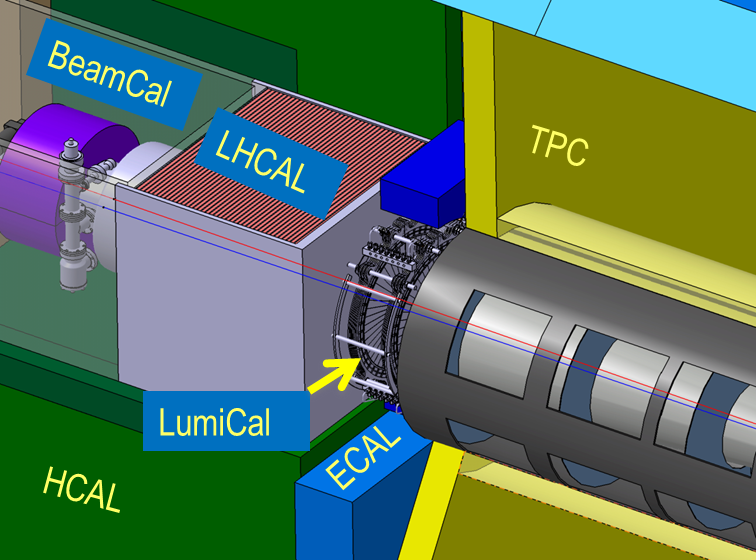
\includegraphics[width=0.45\columnwidth]{Calorimeter/FCAL/figs/forward_region_new} \hfill
   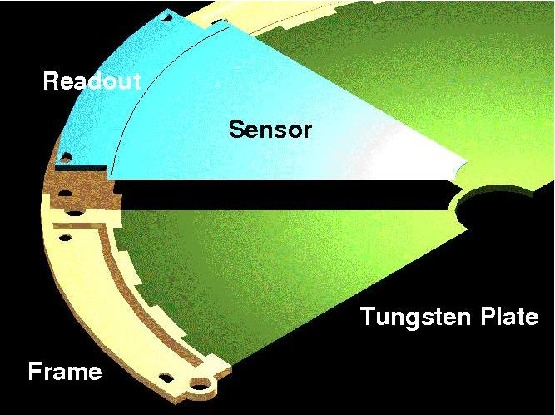
\includegraphics[width=0.45\columnwidth]{Calorimeter/FCAL/figs/BClayer}
  \caption{Left: The very forward region of the ILD detector.
  LumiCal, BeamCal and LHCAL are carried by
  the support tube for the final focusing quadrupole QD0 and the beam-pipe.
  TPC denotes the central track chamber, ECAL the electromagnetic and
  HCAL the hadron calorimeter.
  Right: A half layer of an absorber disk with a sensor sector and front-end electronics.}
  \label{fig:Forward_structure}
\end{figure}
Due to the high occupancy originating from beamstrahlung and two-photon processes,
both calorimeters need a dedicated fast readout.
In addition, the lower polar angle range of BeamCal is exposed to a large flux
of low energy electrons, resulting in depositions up to one
MGy per year. Hence, radiation hard sensors are needed.

\subsection{Mechanical Concept}
Since in both calorimeters a robust electron and photon shower measurement
is essential, a small Moli\`{e}re radius will be preferable.
Compact
cylindrical sandwich
calorimeters using tungsten absorber disks of one radiation length thickness, interspersed with
finely segmented silicon (LumiCal) or GaAs (BeamCal) sensor planes, as sketched in
Figure~\ref{fig:Forward_structure}~(right),
are found
to match the requirements from physics~\cite{2010JInst...512002A}.

\subsection{Recent Milestones}
\subsection{Engineering Challenges}
Engineering challenges within the current and future research within FCAL are the following:
\begin{itemize}
\item{a slim assembled sensor plane. The space between absorber planes must be kept as small
as possible. The fan-out to move the signals from the sensor pads to the outside radius must be very thin and
hence a new connectivity technology must be applied.}
\item{multichannel front-end and ADC ASICs for the prototype.
A compromise must be found between integration, miniaturization and costs}.
\item{operation using \todo{what is the challenge?} power pulsing}.
\item{a dedicated solution for data concentration, \todo{be more specific} data reduction and transmission}.
\item{\todo{be more specific} precise alignment and position monitoring}.
\end{itemize}

\subsection{Future Plans}

\subsubsection{Sensors and ASICs}
Large area GaAs sensors, as shown in Figure~\ref{fig:GaAs}, were developed
and produced in collaboration with partners in industry. The Liquid Encapsulated
Czochralski technology is used. The sensors were
doped by a shallow donor (Sn or Te),
and then compensated  with Chromium.
\begin{figure}[hbp]
\begin{center}
    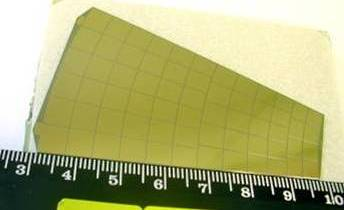
\includegraphics[width=0.8\columnwidth]{Calorimeter/FCAL/figs/GaAs_sensor_new.jpg}
  \end{center}
          \caption{A GaAs pad sensor developed for BeamCal.}
    \label{fig:GaAs}
\end{figure}
This results in a semi-insulating GaAs material with a resistivity of about $\unit[10^7]{\Omega m}$.
The sensors are \unit[0.5]{mm} thick with pads of a few mm$^2$ area. The operation voltage is about \unit[100]{V} with
leakage current per pad less than \unit[500]{nA}.

Prototypes of LumiCal sensors have been designed
and manufactured by Hamamatsu
Photonics.
Their shape is a ring segment of 30$^\circ$.
The thickness of the n-type silicon bulk is \unit[0.320]{mm}.
The pitch of the concentric p$^+$ pads is \unit[1.8]{mm} and
the gap between two pads is \unit[0.1]{mm}.
The bias voltage for full depletion ranges between 39 and \unit[45]{V},
and the leakage currents per pad are below \unit[5]{nA}~\cite{eudet2009}.

Dedicated ASICs were designed choosing
an
architecture~\cite{Boie1982365,Gatti:1986qq}
comprising a charge sensitive amplifier and a shaper.
ASICs, containing 8 front--end channels, were designed and fabricated in $\unit[0.35]{\micron}$ CMOS technology.
A micro-graph of the prototype, glued and bonded on the PCB, is shown Figure~\ref{fig:frontend_photo}.
A variable gain in both the charge amplifier and
the shaper is implemented by a mode switch. The peaking time of the shaper output signal is \unit[60]{ns}.
More results of the measurements of the performance were published elsewhere~\cite{4600902}.
A dedicated low-power, small-area, multichannel ADC is designed and produced~\cite{6156491}.
\begin{figure}[hbp]
\begin{center}
 \begin{tabular}{rrr}
    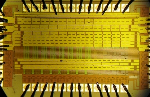
\includegraphics[width=0.4\columnwidth]{Calorimeter/FCAL/figs/fcal_lumical_fe_photo}
     &~~~~~~&
 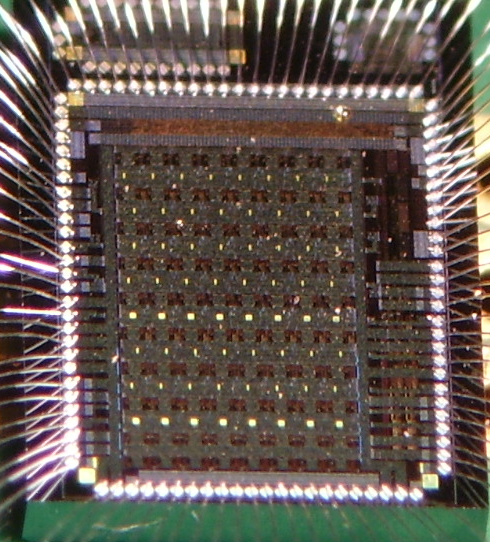
\includegraphics[width=0.4\textwidth,height=0.28\textwidth]{Calorimeter/FCAL/figs/adc_asic_photo.png} \\

\end{tabular}
   \end{center}
          \caption{Left: Micrograph of front--end ASIC.
               Right: Micrograph of ADC ASIC.}
    \label{fig:frontend_photo}
\end{figure}
It comprises eight 10-bit power and frequency (up to \todo{what is MS/s} \unit[24]{MS/s}) scalable pipeline ADCs and the necessary
auxiliary components.
A micro-graph of the prototype is shown in Figure~\ref{fig:frontend_photo}.

A dedicated ASIC development is ongoing for BeamCal~\cite{6200898}
with a special option for a fast readout of an reduced amount of
information from each bunch-crossing to be used for a fast feedback system for beam-tuning.
A prototype of a pixel sensor readout for the pair monitor, positioned in front of BeamCal was designed in \todo{has this been introduced before?}SoI
technology~\cite{Sato201153}.

\subsection{Test-beam Results}
Several test-beam campaigns were done to investigate the performance of single fully instrumented sensor planes,
both for LumiCal and BeamCal.
Prototypes of sensor planes assembled with FE and ADC ASICs,
as shown in Figure~\ref{fig:fcal_lumical_module_photo},
were built using LumiCal and BeamCal sensors~\cite{1748-0221-7-01-T01004}.
\begin{figure}[hbp]
\centering
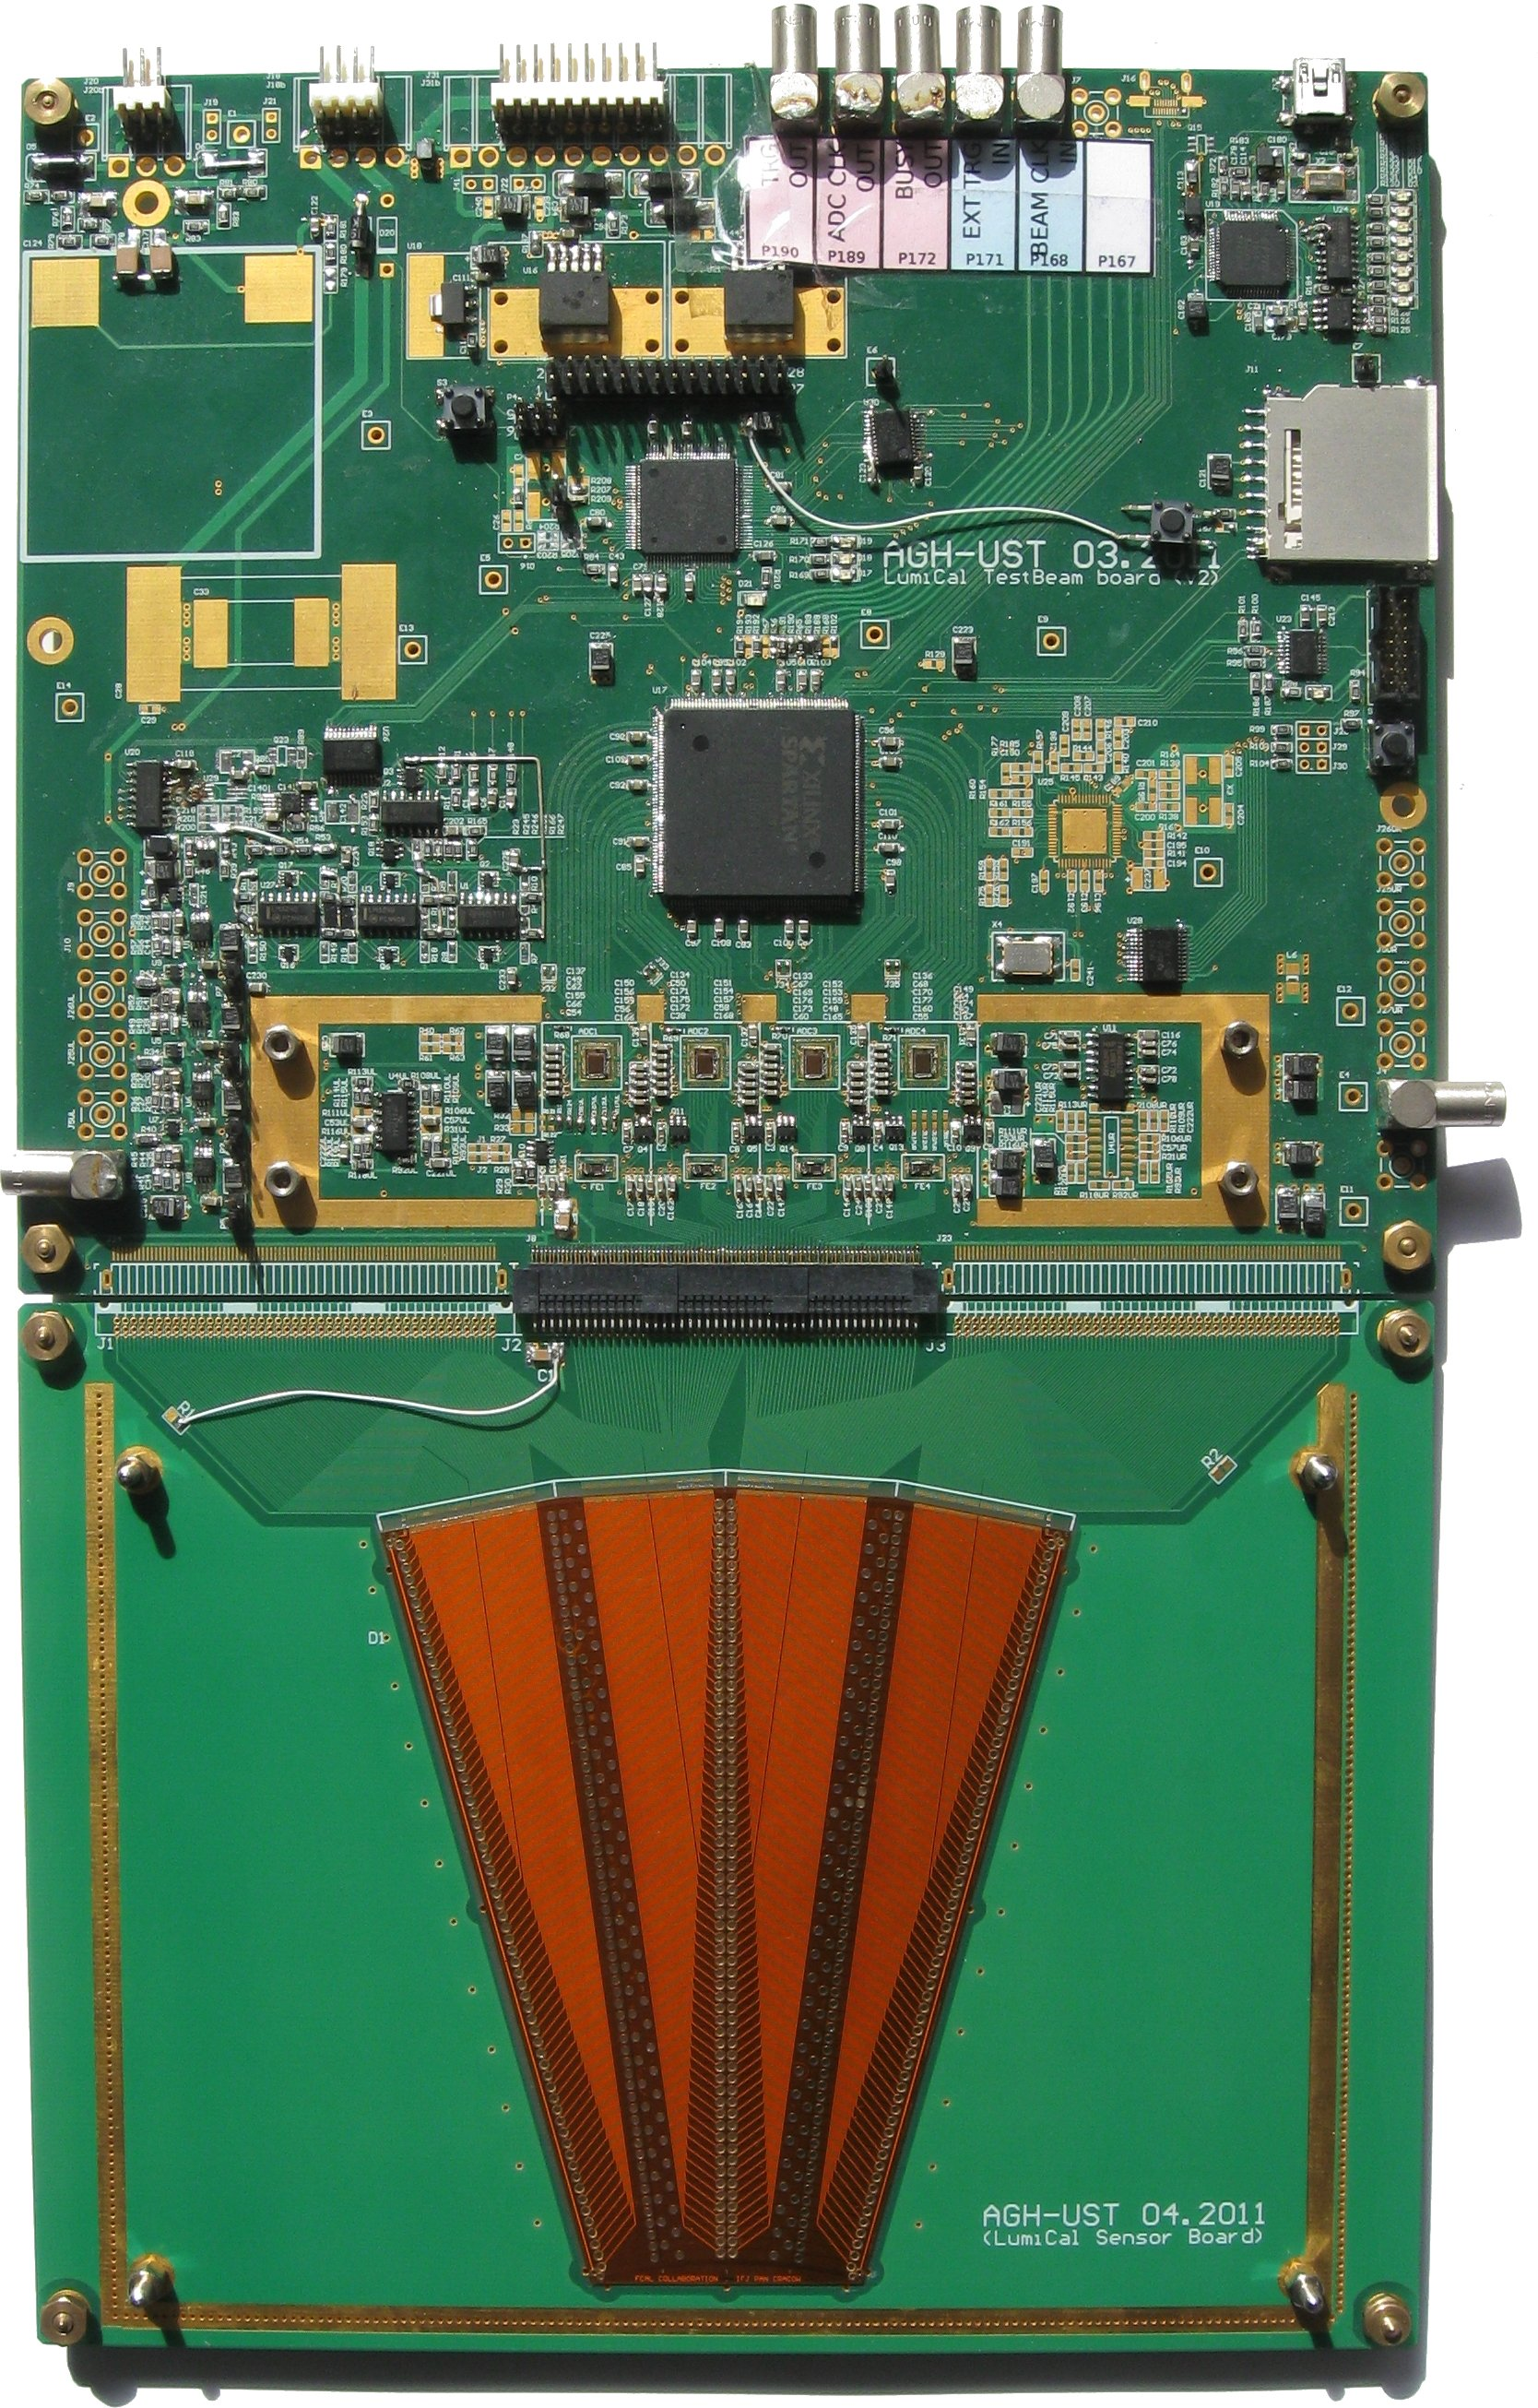
\includegraphics[width=0.35\columnwidth,angle=90]{Calorimeter/FCAL/figs/tb3_complete_module}
\caption{Photograph of LumiCal readout module with sensor connected.}
\label{fig:fcal_lumical_module_photo}
\end{figure}
The detector plane prototypes were installed in an electron beam and
the trajectories of beam particles were measured by four planes of a silicon strip
telescope.
The front-end electronics outputs were sampled synchronously with the
beam clock, a mode used at the ILC.
\begin{figure}[htpb]
\centering
  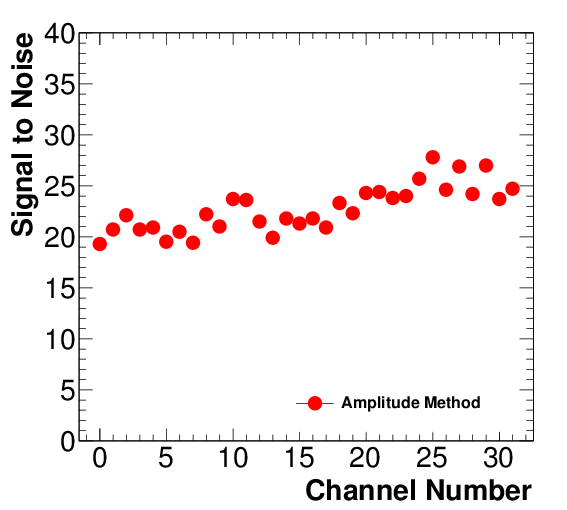
\includegraphics[width=0.45\columnwidth]{Calorimeter/FCAL/figs/StoN_AmplitudeMethod_TB11} \hfill
  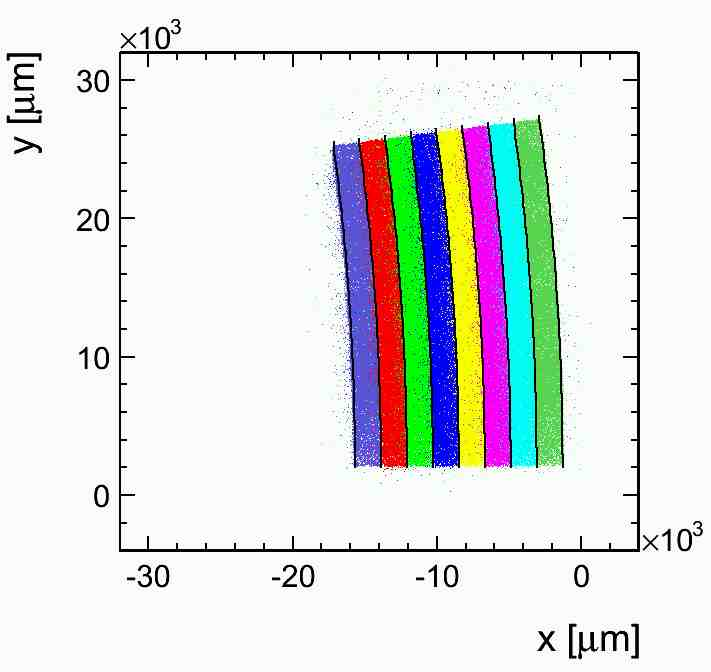
\includegraphics[width=0.45\columnwidth]{Calorimeter/FCAL/figs/hit_map_area1}
  \caption{Left: The signal-to-noise ratio of all readout channels.
          Right: Distribution of the predicted impact points on pads with a color coded signal.}
\label{fig:sinalnoise}
\end{figure}
Data were taken for different pads and also for regions covering pad boundaries.
Signal-to-noise ratios
of better than 20 are measured for beam particles both for LumiCal and BeamCal sensors,
as illustrated in Figure~\ref{fig:sinalnoise}~(left).
The impact point on the sensor is reconstructed from the telescope information.
Using a color code for the signals on the pads
the structure of the sensor becomes nicely visible, as also seen in Figure~\ref{fig:sinalnoise}~(right).
The sensor response was found to be uniform over the pad area and to drop by about 10\% in the
area between pads.

\subsection{Radiation Damage Studies}


Two studies of the radiation tolerance of potential BeamCal sensors have been carried out. The
radiation tolerance of prototype GaAs sensors has been explored by exposing the sensors
to direct irradiation from a high-intensity electron beam of about \unit[10]{MeV}~\cite{sdalinac},
which is an energy expected from beamstrahlung
remnants at the ILC.
It was found that the sensors can be operated up
to approximately \unit[1]{MGy} of this type of radiation without a significant increase in the
leakage current~\cite{1748-0221-7-11-P11022}; however, significant loss in the response to ionizing particles was observed.
In addition, several different silicon-diode sensor technologies were exposed to varying levels
of radiation induced by the SLAC End Station A Test Beam (ESTB).
For this study, the ESTB test beam, with energies
varying between 3 and \unit[11]{GeV}, was directed into a tungsten beam stop.
The beam stop was split at approximately shower-max and the sensor inserted,
leading to an exposure incorporating the full spectrum of particle species that will
irradiate the BeamCal sensors. Both n-type bulk oxygenated float-zone and magnetic Czochralski
detectors were explored, with exposures varying from 0.2 to \unit[2.2]{MGy} as allowed by
the limited exposure rate and
beam availability. It was found that, after allowing for a short period of controlled annealing,
all sensor types withstood the maximum dose that they received with little loss in response
to ionizing particles~\cite{2014arXiv1402.2692B}, but with some increase in leakage current. Further annealing studies,
geared towards achieving a minimal post-irradiation leakage current, continue.
Further irradiation studies in the ESTB are planned for the \todo{update?} spring running periods of 2014 and 2015.
The sensor assessment (``charge-collection efficiency'') apparatus at the Santa Cruz Institute
for Particle Physics is being adapted for the evaluation of pad sensors, which will allow for radiation
damage studies of the prototype GaAs sensors in this realistic electromagnetic shower environment.
Studies to push the silicon diode sensors to higher levels of irradiation are also planned.


\subsection{Technological Prototype}

Currently the goal of FCAL is to prepare a calorimeter prototype for test-beam measurements. These measurements
are essential firstly to develop and test engineering solutions to build a very compact calorimeter and
secondly to verify the results of Monte Carlo studies. Depending on the test beam
results the calorimeter may be redesigned.
For the prototype calorimeter
a mechanical structure, a sufficient amount of front-end and ADC ASICs, FPGAs for
data concentration and
a data acquisition system are needed.

\subsubsection{Mechanical Stack}

A flexible mechanical structure, as shown in  Figure~\ref{fig:mechanical_structure}, has been built as part of the AIDA I project at CERN,
to compose a calorimeter prototype instrumented both with LumiCal and BeamCal sensors. Tungsten absorber plates, glued on a permaglass
frame, are precisely
positioned on a rod assembly, and interspersed with fully assembled sensor planes.
\begin{figure}[hbp]
\centering
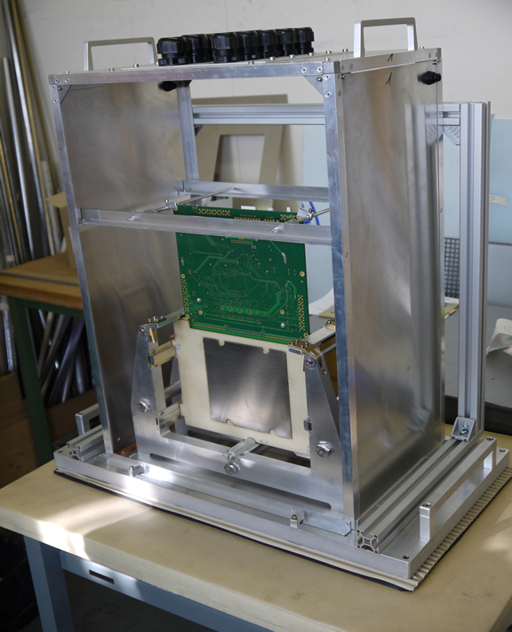
\includegraphics[width=0.6\columnwidth,]{Calorimeter/FCAL/figs/mechanical_structure_2}
\caption{Photograph of the flexible mechanical structure. Tungsten absorber plates, glued on perma-glass frames, are put into slots of the
rod assembly.}
\label{fig:mechanical_structure}
\end{figure}
The flatness of the absorber plates is better than \unit[50]{\micron} to allow high compact packing of sensor and absorber planes.

\subsubsection{Alignment and Position Monitoring }

A laboratory set-up for position monitoring has been constructed by IFJPAN Cracow using semi-transparent
silicon sensors. Test measurements demonstrated that position monitoring with \micron precision is possible.

\subsubsection{Front-End and ADC ASICs}


To match the requirements of extremely low power consumption and taking into account possible radiation
fields in the very forward region, a new development of the front-end and ADC ASICs in deep sub-micron
\unit[130]{nm} CMOS technology has been
pursued within AIDA by UST Cracow.
These ASICs will be sufficiently fast to be used both in LumiCal and BeamCal.
The overall readout architecture, so far successfully produced in \unit[350]{nm} CMOS technology and used in the test-beam
measurements as described above, has not been changed and comprises separated front-end
and ADC ASICs for each readout channel.
\begin{figure}[hbp]
\centering
    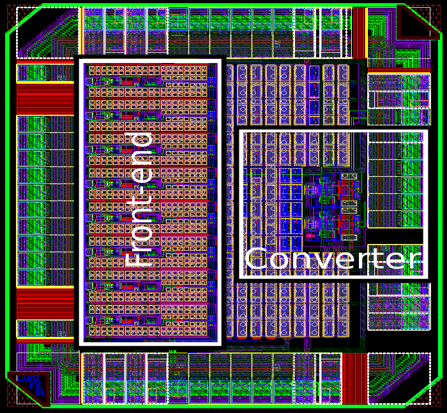
\includegraphics[width=0.45\textwidth]{Calorimeter/FCAL/figs/FE_ASIC.png} \hfill
	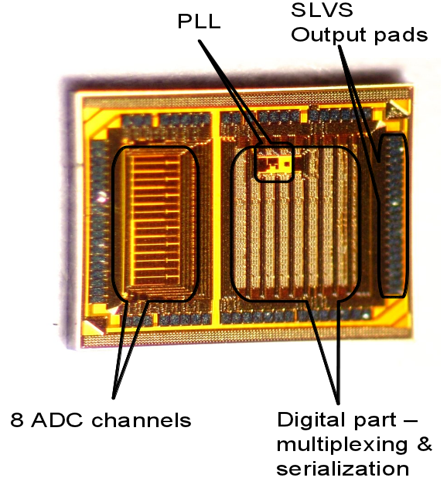
\includegraphics[width=0.45\textwidth]{Calorimeter/FCAL/figs/ADC_ASIC_2.png}
	\caption{Left: 8 channel FE ASIC in \unit[130]{nm} technology.
		 	 Right: ADC ASIC in \unit[130]{nm} technology.}
    \label{fig:ASIC_ADC}
\end{figure}
For both FE and ADC ASICs prototypes, shown in Figure~\ref{fig:ASIC_ADC}, are under test.

\subsubsection{Data Concentrator and DAQ}

In order to operate a large amount of sensor planes the readout has to be orchestrated.
For this purpose a FPGA based data concentrator is foreseen
which may deliver data in the so called AIDA protocol. The design of this device is currently under discussion.
The higher level DAQ will depend on the functionality of the data concentrator.
For the readout of test-beam data we have software, mainly developed by University of Tel Aviv,
which can be easily adopted.
For a final device FCAL will follow the developments of a common DAQ for all subdetetors.


\subsection{Applications Outside of Linear Colliders}

The expertise acquired within FCAL for radiation hard sensors and fast front-end electronics was
used to build, commission and operate fast
beam-conditions monitors at the CMS experiment at LHC.
Radiation hard sensors developed within FCAL are used as beam-loss monitors
with excellent time resolution at FLASH and LHC. A design for beam-loss monitors for XFEL is prepared.
In addition, front-end ASICs are under development for the upgrade of the LHCb tracker.
